\documentclass[11pt,a4paper]{article}
\usepackage[utf8]{inputenc}
\usepackage[T1]{fontenc}
\usepackage[spanish,es-noquoting]{babel}
\usepackage{amsmath,amssymb}
\usepackage{graphicx}
\usepackage{booktabs}
\usepackage{float}
\usepackage{listings}
\usepackage{xcolor}
\usepackage{caption}
\usepackage[margin=2.4cm]{geometry}
\usepackage{hyperref}
\hypersetup{colorlinks=true,linkcolor=blue!50!black,urlcolor=blue!50!black}

\definecolor{codegray}{gray}{0.95}
\definecolor{commentgreen}{rgb}{0.0,0.5,0.0}
\definecolor{keywordblue}{rgb}{0.0,0.0,0.6}
\definecolor{stringmauve}{rgb}{0.58,0.0,0.82}
\lstset{
  language=Matlab, basicstyle=\ttfamily\footnotesize,
  backgroundcolor=\color{codegray}, commentstyle=\color{commentgreen}\itshape,
  keywordstyle=\color{keywordblue}\bfseries, stringstyle=\color{stringmauve},
  numbers=left, numberstyle=\tiny\color{gray}, numbersep=6pt,
  frame=single, rulecolor=\color{gray!40}, breaklines=true,
  columns=fullflexible, showstringspaces=false, captionpos=b,
  xleftmargin=14pt, framexleftmargin=14pt
}
\newcommand{\code}[1]{\texttt{\small #1}}

\begin{document}

% ================= DATOS =================
\section{Datos generales}
\begin{center}
\renewcommand{\arraystretch}{1.3}
\begin{tabular}{ll}
\toprule
\textbf{Curso} & Inteligencia Artificial Aplicada al Control (ICA636-0001) \\
\textbf{Trabajo} & Tarea 4 --- Control de Sistemas Dinámicos \\
\textbf{Alumno} & Joel Arzapalo Guerra \\
\textbf{Código} & 20032006 \\
\textbf{Fecha} & \today \\
\bottomrule
\end{tabular}
\end{center}
\vspace{0.5cm}

% ================= INTRODUCCION =================
\section{Introducción}
Este trabajo analiza un conjunto de programas MATLAB que entrenan una red neuronal
para actuar como \textbf{controlador} (neurocontrolador) de un sistema dinámico. El
controlador recibe el estado (o su error respecto de una referencia) y produce la señal
de control $u$ que se aplica a la planta. La planta común es un sistema discreto
\textbf{bilineal} de 2 estados:
\[
  x(k{+}1) = A\,x(k) + B\,u(k) + \big(G\,x(k)\big)\,u(k) \;[+\,W\,\text{pert}],
\]
donde el término $(Gx)u$ es una ganancia de entrada dependiente del estado.

El código implementa las dos estrategias de aprendizaje de la Clase 9, que se distinguen
por \emph{cómo se calcula el gradiente del costo} a través de la dinámica de la planta:

\begin{itemize}
  \item \textbf{Aprendizaje estático} (\code{DynamicBPControlEstaticoModelo0/1/3.m}):
        el gradiente usa solo la sensibilidad \emph{instantánea} del estado siguiente al
        control, \code{dxdu = B + G*x}. No considera la dinámica de lazo cerrado; es
        simple y adecuado para \textbf{plantas estables} (mejorar el transitorio,
        regulación y seguimiento).
  \item \textbf{Aprendizaje dinámico (DBP, \emph{Dynamic Back Propagation})}
        (\code{DynamicBPControl2/2a/2b.m}): el gradiente se propaga
        \emph{recursivamente en el tiempo} a través del jacobiano del lazo cerrado. Es más
        costoso pero necesario para \textbf{plantas inestables}.
\end{itemize}

El costo minimizado es $J=\tfrac12\sum_k (x_k-x_k^*)^{\top}Q(x_k-x_k^*) + R\,u_k^2$,
con $Q=\mathrm{diag}(q_1,q_2)$ y $R$ el peso del esfuerzo de control.

El informe cubre (i) el \textbf{análisis del código} de los seis scripts y (ii) los
\textbf{resultados experimentales}, entrenando los controladores y estudiando la
influencia de los parámetros (peso $R$, número de neuronas, grado de inestabilidad,
realimentación parcial, perturbaciones externas y ruido de medición). Los scripts
originales (interactivos, con \code{input()} y \code{load} de pesos) se adaptaron a
versiones no interactivas (\code{rng} fijo, hiperparámetros en código),
encapsulando el entrenamiento en las funciones \code{train\_static\_ctrl.m} y
\code{train\_bptt\_ctrl.m}, fieles a la matemática de los originales.

% ================= ANALISIS DE CODIGO =================
\section{Análisis del código}

\subsection{Estructura común}
Todos los scripts comparten el mismo esqueleto por celdas \code{\%\%}: definición de la
planta ($A,B,G,W$), condiciones iniciales \code{x\_ini} (una columna por caso, el código
deduce \code{nini=size(x\_ini,2)}), arquitectura de la red (\code{ne} entradas,
\code{nm=50} neuronas, salida escalar $u$), carga de pesos, bucle de entrenamiento y
visualización (una figura por condición inicial). La activación oculta es la sigmoide
bipolar $n=2/(1+e^{-(m-c)/a})-1$ con $m=v^{\top}\text{in\_red}$, y el control es
$u=w^{\top}n + u^*$ (con $u^*$ la \emph{acción anticipativa} de equilibrio).

\subsection{Familia estática: \texttt{...EstaticoModelo0/1/3.m}}
\textbf{Modelo0} (único que \emph{entrena}) regula al origen una planta \emph{estable}.
La clave es que el gradiente comparte un mismo coeficiente escalar por paso:

\begin{lstlisting}[caption={Gradiente estático: solo el término instantáneo \texttt{dxdu}.}]
dxdu = B + G*x;                 % sensibilidad d x(k+1)/d u
er  = (x - out_des);            % error de seguimiento
erq = q .* er;
g   = erq'*dxdu + R*u(k,j);     % coeficiente escalar retropropagado
dJdw_t = dJdw_t + g*dudw_s;     % mismo g para w, v, c, a
dJdv_t = dJdv_t + g*dudv_s;
\end{lstlisting}

Incorpora \textbf{momento} (\code{alpha=0.95}) y guarda los \emph{mejores} pesos vistos
(el costo puede oscilar con $\eta$ alto). \textbf{Modelo1} y \textbf{Modelo3} \emph{no}
entrenan: cargan \code{redcontrolestatico0} y validan el mismo controlador para
\emph{seguimiento} de una consigna con \emph{acción anticipativa} (\code{in\_red=x-r},
\code{u=red+uast}) y para \emph{robustez} ante variaciones de la planta (nominal, $A$
menos estable, $B$ a la mitad, $G$ duplicada), respectivamente.

\subsection{Familia dinámica (DBP): \texttt{DynamicBPControl2/2a/2b.m}}
\textbf{Control2} estabiliza una planta \emph{inestable} ($A$ con diagonal $>1$). El
gradiente es retropropagación en el tiempo: se mantienen acumuladores recursivos de las
sensibilidades del estado a los parámetros, actualizados con el jacobiano del lazo
cerrado:

\begin{lstlisting}[caption={Recursión DBP vectorizada (jacobiano del lazo cerrado).}]
jacob   = A + u(k,j).*G;    % jacobiano de la planta  d x(k+1)/d x
dxdu    = B + G*x;          % d x(k+1)/d u
dudx    = w'*dndm*v';       % d u/d x  (sensibilidad del control al estado)
jacob_t = dxdu*dudx + jacob;               % jacobiano del lazo cerrado
Sw_t = dudw_s*dxdu' + Sw_t*jacob_t';       % S_p(k+1)=du/dp*dxdu' + S_p(k)*jacob_t'
\end{lstlisting}

La recursión está \textbf{vectorizada} (matrices \code{Sw\_t}, \code{Sv\_t}, \dots
indexadas por estado) y se actualiza de forma \emph{simultánea} para todos los estados.
\textbf{Control2a} usa realimentación \emph{parcial}: la entrada de la red es una salida
medida $y=Cx$ (\code{ne=1}); documenta que $C=[0\ 1]$ (medir $x_2$) controla, pero
$C=[1\ 0]$ (medir $x_1$) no. \textbf{Control2b} valida el rechazo de \emph{perturbaciones}
(consigna activa $x^*_1=1$, perturbación senoidal por $W=[0;1]$, y \emph{ruido de
medición} $0.005\,\mathcal{N}$ sumado a \code{in\_red}).

\paragraph{Nota sobre la realimentación parcial.} En la versión no interactiva, la sensibilidad
del control al estado se propaga correctamente incluyendo la matriz de salida,
\code{dudx = (w'*dndm*v')*C}, que para $C=I$ (estado completo) recupera exactamente la
expresión de \code{Control2}.

% ================= RESULTADOS =================
\section{Resultados experimentales}
Resultados con las versiones no interactivas (semilla fija). Las figuras se generan con
\code{Informe/exp/run\_all.m}.

\subsection{Control estático: regulación en planta estable}
\label{sec:C1}
Se entrenó el neurocontrolador estático ($n_m=50$, $\eta=2$, momento $0.95$) para regular
al origen la planta estable, partiendo de 4 condiciones iniciales. El costo converge
(Fig.~\ref{fig:C1conv}) y el lazo cerrado lleva ambos estados a cero con una señal de
control suave (Fig.~\ref{fig:C1resp}); el error final es prácticamente nulo
($\sim10^{-13}$) en las 4 condiciones. Frente al sistema \emph{sin} control, el
neurocontrolador \textbf{acelera notablemente el transitorio} (Fig.~\ref{fig:C1unc}),
que es justamente el objetivo de mejora de respuesta del PDF.

\begin{figure}[H]
\centering
\begin{minipage}{0.32\linewidth}\centering
  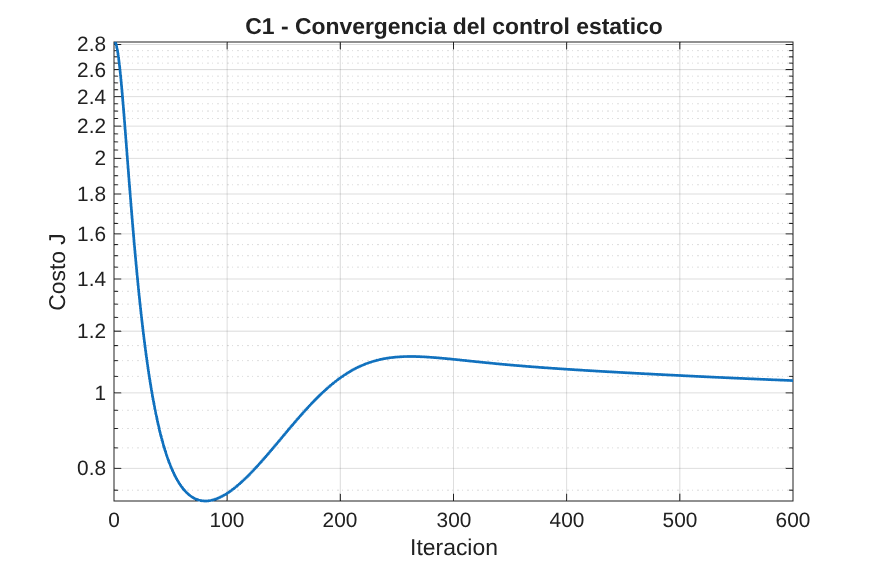
\includegraphics[width=\linewidth]{figs/C1_conv.png}
  \caption{Convergencia del costo.}\label{fig:C1conv}
\end{minipage}\hfill
\begin{minipage}{0.32\linewidth}\centering
  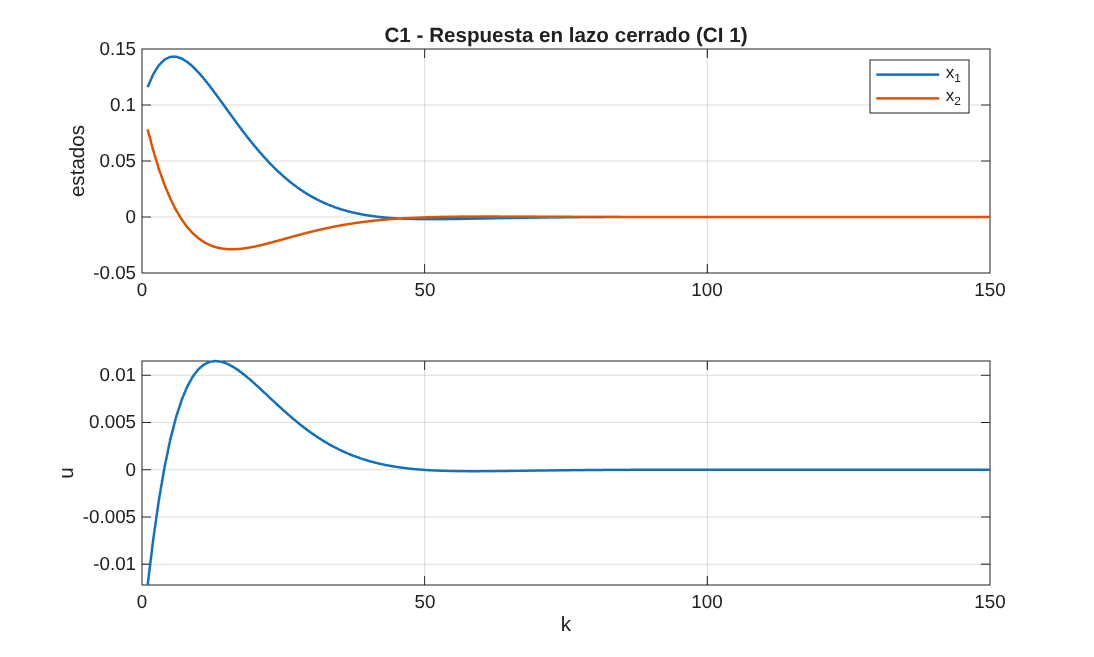
\includegraphics[width=\linewidth]{figs/C1_response.png}
  \caption{Respuesta en lazo cerrado.}\label{fig:C1resp}
\end{minipage}\hfill
\begin{minipage}{0.32\linewidth}\centering
  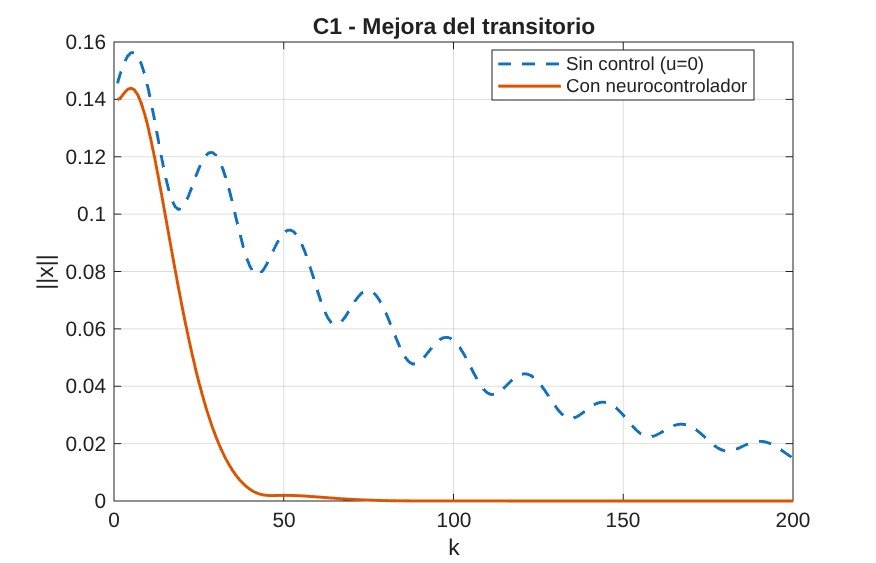
\includegraphics[width=\linewidth]{figs/C1_vs_uncontrolled.png}
  \caption{Con vs sin control.}\label{fig:C1unc}
\end{minipage}
\end{figure}

\paragraph{Peso $R$, neuronas y generalización.}
Como la planta es estable y fácil de regular, el error final permanece despreciable para
todo $R$ ensayado (Fig.~\ref{fig:C1R}); el peso $R$ solo influye levemente en el esfuerzo
de control ($\Sigma u^2\!\approx\!0.0021$, subiendo a $0.0042$ con $R=1$). El número de
neuronas tiene efecto modesto sobre el costo (Fig.~\ref{fig:C1nm}). Lo más destacable es
la \textbf{generalización}: entrenado con condiciones iniciales pequeñas, el controlador
regula igualmente bien condiciones \textbf{hasta $20\times$ mayores}, con error final
$\sim10^{-12}$ (Fig.~\ref{fig:C1gen}).

\begin{figure}[H]
\centering
\begin{minipage}{0.32\linewidth}\centering
  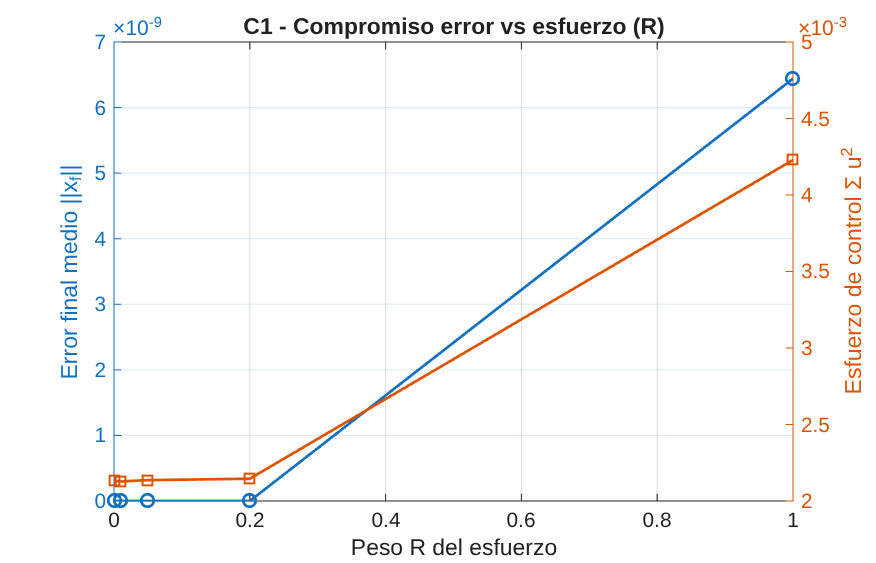
\includegraphics[width=\linewidth]{figs/C1_R.png}
  \caption{Compromiso error/esfuerzo vs $R$.}\label{fig:C1R}
\end{minipage}\hfill
\begin{minipage}{0.32\linewidth}\centering
  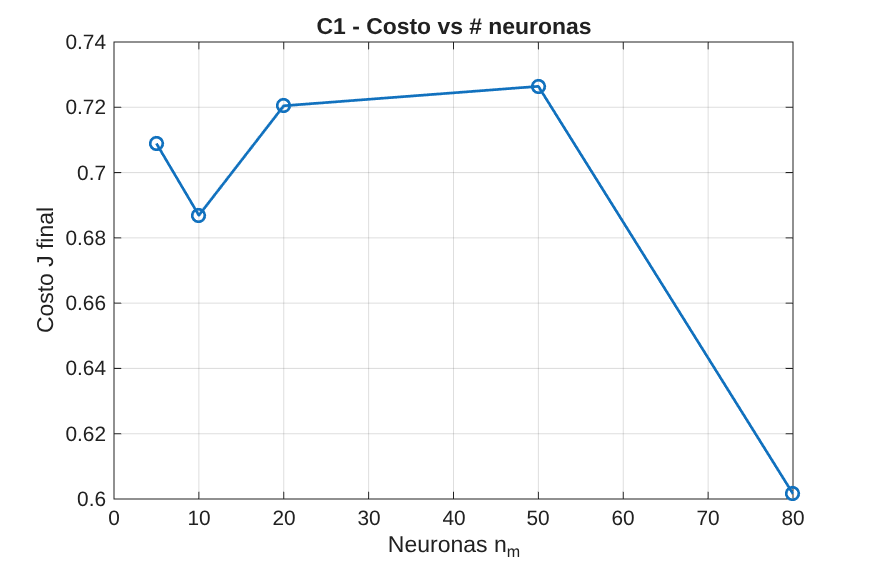
\includegraphics[width=\linewidth]{figs/C1_neurons.png}
  \caption{Costo vs $n_m$.}\label{fig:C1nm}
\end{minipage}\hfill
\begin{minipage}{0.32\linewidth}\centering
  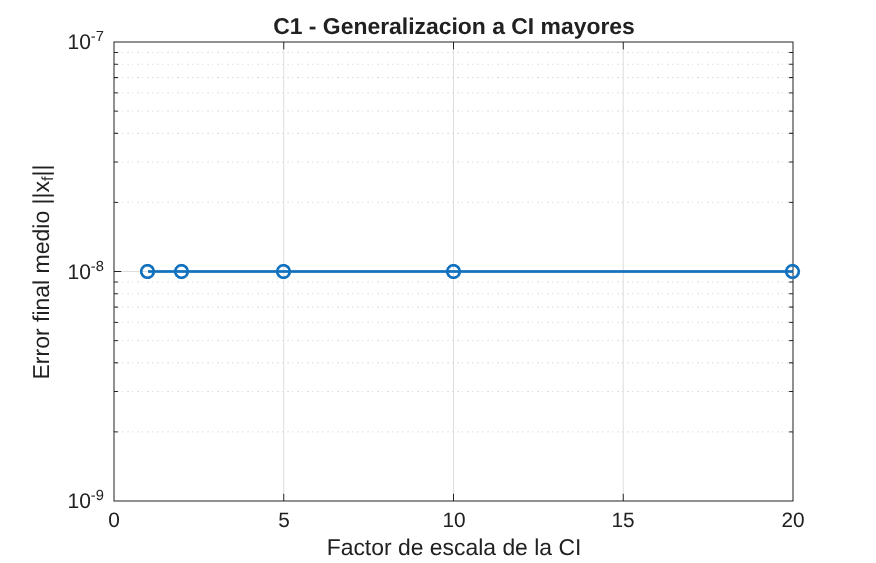
\includegraphics[width=\linewidth]{figs/C1_gen.png}
  \caption{Generalización a CI mayores.}\label{fig:C1gen}
\end{minipage}
\end{figure}

\subsection{Robustez y rechazo de perturbaciones (estático)}
\label{sec:C2}
Se aplicó el \emph{mismo} controlador entrenado en la planta nominal a cuatro variantes
de planta (Modelo3): nominal, $A$ menos estable, ganancia $B$ reducida al 50\% y término
bilineal $G$ duplicado. En los cuatro casos el lazo cerrado \textbf{sigue estabilizando}
(Fig.~\ref{fig:C2rob}, todas las trayectorias $\|x\|\to0$): el neurocontrolador es
robusto a estas variaciones sin reentrenar.

Para el rechazo de perturbaciones (Modelo1, seguimiento de $x^*_1=0.1$ con
\emph{acción anticipativa}), se inyectó una perturbación senoidal externa de amplitud creciente.
El error de seguimiento en régimen permanente crece de forma \textbf{proporcional} a la
amplitud (Tabla~\ref{tab:C2}, Fig.~\ref{fig:C2dist}): el controlador \emph{atenúa} la
perturbación pero, al ser un control estático sin acción integral, no la cancela por
completo.

\begin{table}[H]\centering
\caption{Error de seguimiento en régimen permanente vs amplitud de la perturbación.}
\label{tab:C2}
\begin{tabular}{lcccc}
\toprule
Amplitud perturbación & 0 & 0.02 & 0.10 & 0.50 \\
Error r.p. $\|x-r\|$ & $1.3\!\times\!10^{-5}$ & 0.0019 & 0.0093 & 0.046 \\
\bottomrule
\end{tabular}
\end{table}

\begin{figure}[H]
\centering
\begin{minipage}{0.48\linewidth}\centering
  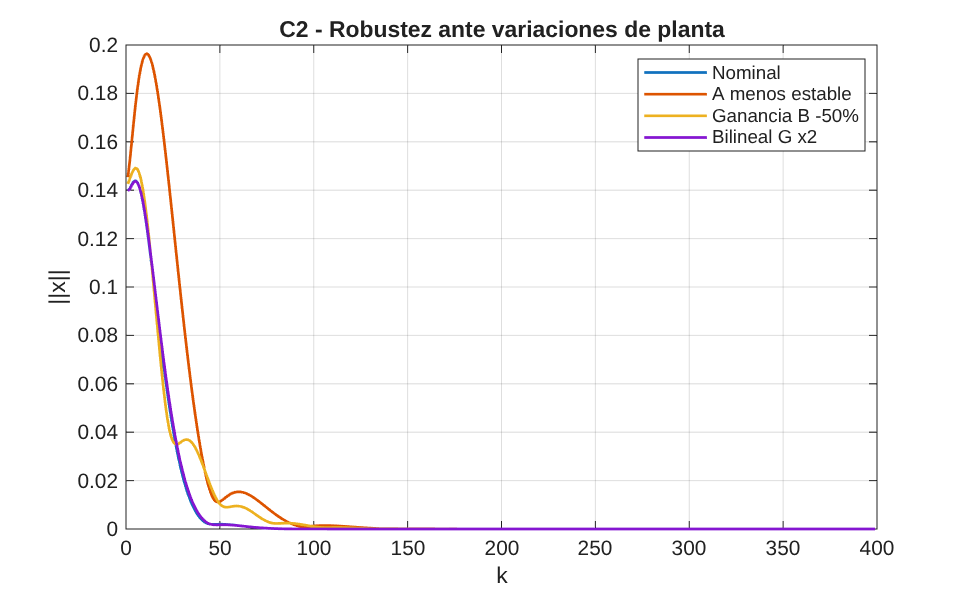
\includegraphics[width=\linewidth]{figs/C2_robust.png}
  \caption{Robustez ante variaciones de planta.}\label{fig:C2rob}
\end{minipage}\hfill
\begin{minipage}{0.48\linewidth}\centering
  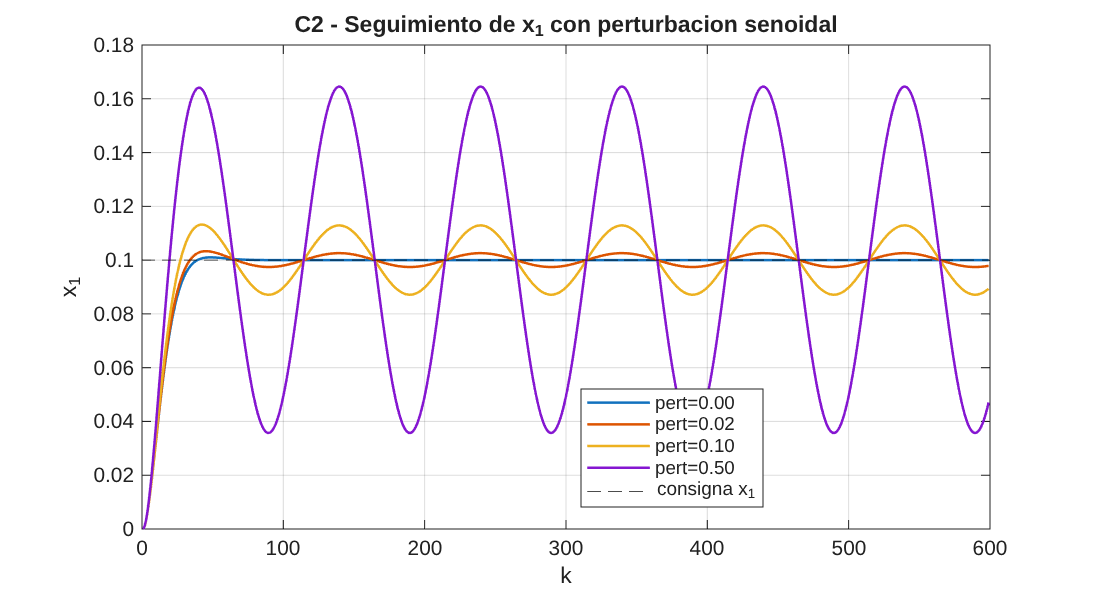
\includegraphics[width=\linewidth]{figs/C2_disturb.png}
  \caption{Seguimiento con perturbación senoidal.}\label{fig:C2dist}
\end{minipage}
\end{figure}

\subsection{Estático vs dinámico en planta inestable}
\label{sec:C3}
Este es el experimento central. Se barrió la inestabilidad de la planta (diagonal de $A$
de $0.98$ a $1.20$) y, en cada nivel, se entrenó un controlador \textbf{estático}
(desde cero) y uno \textbf{dinámico DBP} (incremental, con arranque desde pesos previos del
nivel previo). Se mide el error final medio $\|x_f\|$: valores $\gg 0.1$ indican que el
lazo cerrado \emph{no} se estabiliza.

El resultado (Tabla~\ref{tab:C3}, Fig.~\ref{fig:C3sweep}) es contundente: el control
estático solo funciona mientras la planta es estable ($0.98$); \textbf{en cuanto la
planta se vuelve inestable ($\ge 1.02$), diverge} (errores de $10^{3}$ a $10^{23}$),
porque su gradiente ignora la dinámica de lazo cerrado. El control dinámico DBP, en
cambio, \textbf{estabiliza todos los niveles} hasta $A_{ii}=1.20$ con error
$\sim10^{-10}$. La Fig.~\ref{fig:C3resp} muestra la respuesta en la planta más inestable:
el estado del sistema con control estático explota mientras el DBP lo lleva al origen.
Esto confirma la tesis de la Clase 9: el aprendizaje estático no sirve para plantas
inestables; se requiere el dinámico.

\begin{table}[H]\centering
\caption{Error final $\|x_f\|$ según el grado de inestabilidad (diagonal de $A$).}
\label{tab:C3}
\begin{tabular}{lcccccc}
\toprule
Diagonal de $A$ & 0.98 & 1.02 & 1.06 & 1.10 & 1.15 & 1.20 \\
\midrule
Estático & $7\!\times\!10^{-12}$ & $1.9\!\times\!10^{3}$ & $7\!\times\!10^{9}$ & $5\!\times\!10^{15}$ & $1.5\!\times\!10^{23}$ & $1.1\!\times\!10^{3}$ \\
Dinámico (DBP) & $3\!\times\!10^{-11}$ & $3\!\times\!10^{-10}$ & $2\!\times\!10^{-10}$ & $7\!\times\!10^{-11}$ & $5\!\times\!10^{-11}$ & $9\!\times\!10^{-12}$ \\
\bottomrule
\end{tabular}
\end{table}

\begin{figure}[H]
\centering
\begin{minipage}{0.48\linewidth}\centering
  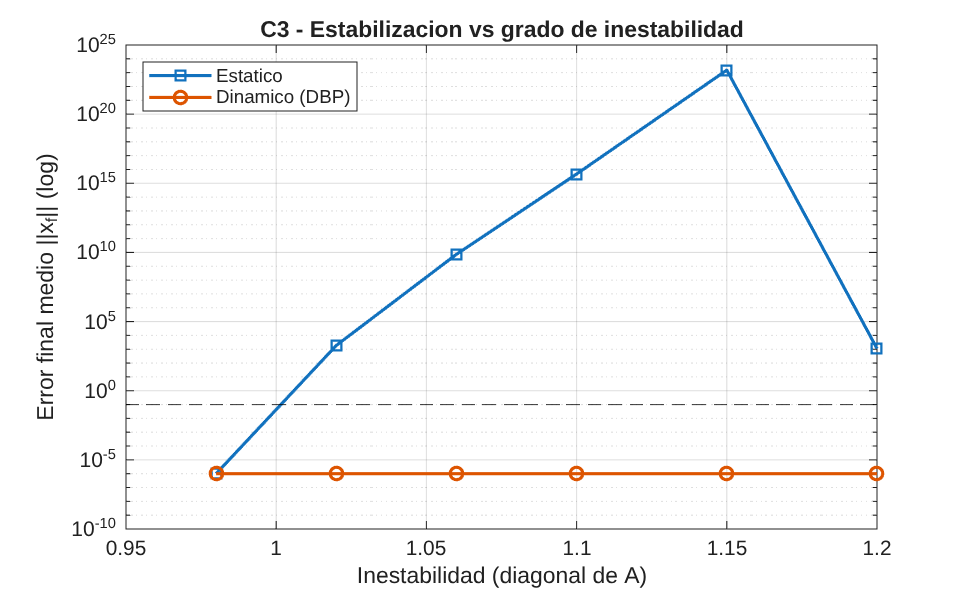
\includegraphics[width=\linewidth]{figs/C3_sweep.png}
  \caption{Estabilización vs grado de inestabilidad.}\label{fig:C3sweep}
\end{minipage}\hfill
\begin{minipage}{0.48\linewidth}\centering
  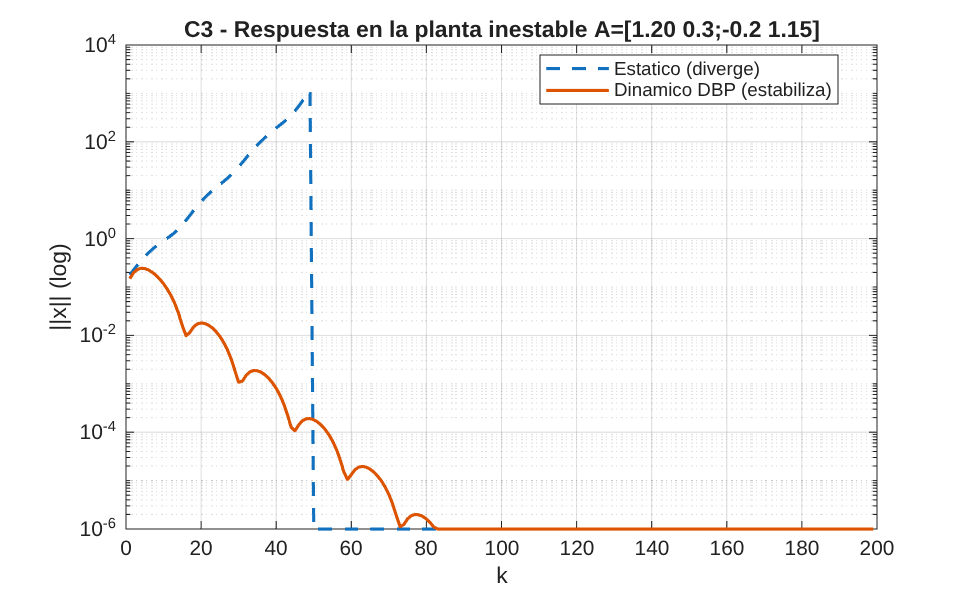
\includegraphics[width=\linewidth]{figs/C3_response.png}
  \caption{Respuesta en $A_{ii}=1.20$ (escala log).}\label{fig:C3resp}
\end{minipage}
\end{figure}

\subsection{Control dinámico DBP: realimentación parcial, perturbaciones y ruido}
\label{sec:C4}
Todos los controladores DBP de esta sección se entrenaron mediante \textbf{entrenamiento por etapas}
(aprendizaje incremental subiendo la inestabilidad con arranque desde pesos previos). En efecto,
un hallazgo del trabajo es que entrenar DBP \emph{desde cero} sobre una planta muy
inestable no converge; el entrenamiento por etapas —tal como emplean los scripts originales
(\code{load} incremental)— es esencial.

\paragraph{Realimentación completa vs parcial.}
Con realimentación \textbf{completa} del estado, el DBP estabiliza la planta inestable
con error $\sim10^{-15}$ (Fig.~\ref{fig:C4part}). Con realimentación \textbf{parcial}
(una sola salida medida $y=Cx$, $ne=1$), el problema es mucho más difícil: entrenando
desde cero (con entrenamiento por etapas), \emph{ninguno} de los controladores de una sola salida
estabilizó la planta inestable dentro del presupuesto de entrenamiento, y su respuesta
diverge. Esto es coherente con \code{Control2a}, que sí logra estabilizar midiendo $x_2$
($C=[0\ 1]$) pero \emph{solo} partiendo de pesos preentrenados (\emph{arranque desde pesos previos}
extenso, \code{load redcontrol2a}) y descarta medir $x_1$ ($C=[1\ 0]$). La conclusión
práctica es doble: reducir la información medida degrada drásticamente la estabilización
por realimentación de salida, y su entrenamiento exige un buen punto de partida.

\paragraph{Rechazo de perturbaciones.}
El regulador DBP sobre la planta más inestable ($A_{ii}=1.20$) mantiene el estado en el
origen; al inyectar una perturbación senoidal externa de amplitud creciente, el error en
régimen permanente crece de forma proporcional (Tabla~\ref{tab:C4}, Fig.~\ref{fig:C4dist}):
sin perturbación regula de forma exacta ($\sim10^{-15}$) y con amplitud $0.1$ el error se
mantiene acotado ($\approx 0.58$), sin desestabilizarse.

\paragraph{Ruido de medición.}
Entrenando con ruido de medición sumado a la entrada de la red (como en \code{Control2b}),
el controlador resultante regula igual de bien que sin ruido: el error final permanece
en $\sim2\times10^{-14}$ para todos los niveles de ruido ensayados
(Fig.~\ref{fig:C4noise}). El DBP es \textbf{robusto al ruido de medición} durante el
entrenamiento, pues el gradiente promediado sobre el horizonte y las condiciones
iniciales atenúa su efecto.

\begin{table}[H]\centering
\caption{Error en régimen permanente del regulador DBP vs amplitud de la perturbación.}
\label{tab:C4}
\begin{tabular}{lccccc}
\toprule
Amplitud perturbación & 0 & 0.01 & 0.03 & 0.05 & 0.10 \\
Error r.p. $\|x\|$ & $10^{-15}$ & 0.055 & 0.166 & 0.278 & 0.577 \\
\bottomrule
\end{tabular}
\end{table}

\begin{figure}[H]
\centering
\begin{minipage}{0.32\linewidth}\centering
  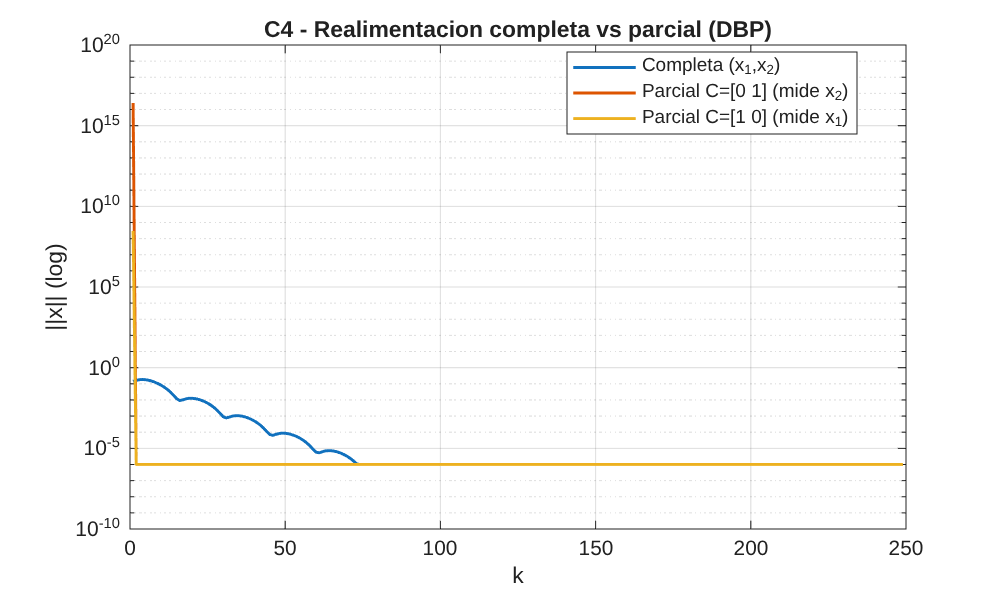
\includegraphics[width=\linewidth]{figs/C4_partial.png}
  \caption{Completa vs parcial.}\label{fig:C4part}
\end{minipage}\hfill
\begin{minipage}{0.32\linewidth}\centering
  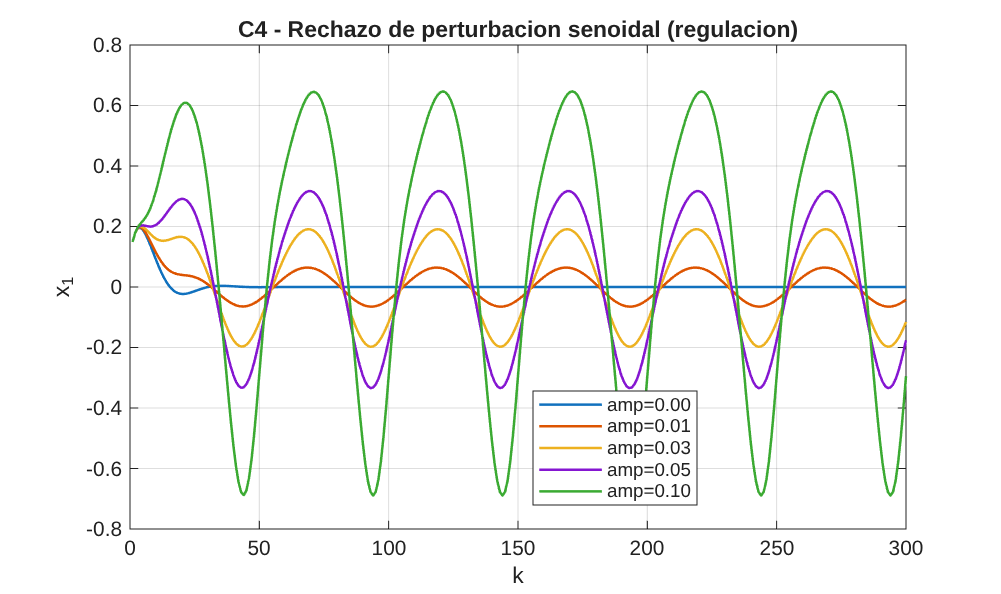
\includegraphics[width=\linewidth]{figs/C4_disturb.png}
  \caption{Rechazo de perturbación.}\label{fig:C4dist}
\end{minipage}\hfill
\begin{minipage}{0.32\linewidth}\centering
  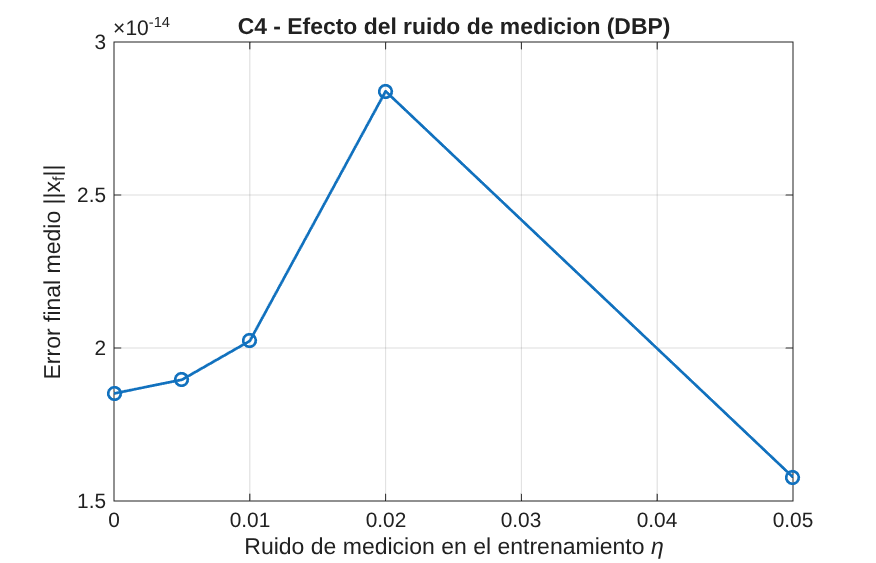
\includegraphics[width=\linewidth]{figs/C4_noise.png}
  \caption{Efecto del ruido.}\label{fig:C4noise}
\end{minipage}
\end{figure}

% ================= CONCLUSIONES =================
\section{Conclusiones}
\begin{enumerate}
  \item \textbf{El aprendizaje estático basta para plantas estables} (Sec.~\ref{sec:C1}):
  el neurocontrolador regula al origen con error despreciable, mejora fuertemente el
  transitorio frente al sistema sin control y \emph{generaliza} a condiciones iniciales
  hasta $20\times$ mayores que las de entrenamiento.

  \item \textbf{El controlador estático es robusto y atenúa perturbaciones}
  (Sec.~\ref{sec:C2}): estabiliza variantes de la planta (nominal, menos estable, $B$ a
  la mitad, $G$ duplicada) sin reentrenar, y el error de seguimiento crece de forma
  proporcional a la amplitud de la perturbación, aunque —al no tener acción integral— no
  la cancela por completo.

  \item \textbf{Para plantas inestables el aprendizaje estático falla y el dinámico es
  imprescindible} (Sec.~\ref{sec:C3}): apenas la planta se vuelve inestable el control
  estático diverge, mientras que el DBP la estabiliza en todo el rango
  ($A_{ii}$ hasta $1.20$) con error $\sim10^{-10}$. Es el resultado central y confirma la
  tesis de la Clase 9.

  \item \textbf{El entrenamiento DBP requiere hacerse por etapas} (aprendizaje incremental de
  la inestabilidad con arranque desde pesos previos): entrenarlo de golpe sobre una planta muy
  inestable no converge.

  \item \textbf{La realimentación parcial es mucho más exigente} (Sec.~\ref{sec:C4}):
  con el estado completo el DBP estabiliza fácilmente, pero con una sola salida medida
  el entrenamiento desde cero no lo logra y requiere un buen punto de partida
  (\emph{arranque desde pesos previos}), como hace el script original. Además, el DBP rechaza
  perturbaciones acotadas y es \emph{robusto al ruido de medición} durante el
  entrenamiento.
\end{enumerate}

\appendix
\section{Archivos del proyecto}
Los experimentos se ejecutan con \code{Informe/exp/run\_all.m}. Las rutinas de
entrenamiento son \code{train\_static\_ctrl.m} (gradiente estático, con momento y
mejores pesos) y \code{train\_bptt\_ctrl.m} (retropropagación en el tiempo vectorizada,
con soporte de realimentación parcial vía la matriz $C$, perturbación y ruido). Cada
experimento C1--C4 guarda sus figuras en \code{Informe/figs/} y sus métricas en
\code{*\_metrics.mat}.

\end{document}
